% TeXplates/Mathematics.tex
% v0.2.2
% https://github.com/HoyanMok/TeXplates
\documentclass[openany, a5paper, oneside]{book} 
% \documentclass{ctexbook} 如果用中文
% \documentclass[10pt,a4paper]{ctexart}  字体大小和纸张大小,默认分别为10pt和letterpaper
% 五号 = 10.5pt,小四=12pt,四号=14pt
% 其他可选参量如twocolumn, 两行排版

\usepackage{../TeXplatesMathematics}
\addbibresource{Lie.bib} % 把这里改成实际的文件名

% 文章标题页信息:
\title{Group Theory}
\author{Hoyan Mok\thanks{E-mail: victoriesmo@hotmail.com}}
\date{\today} % 自动生成日期
\titlepic{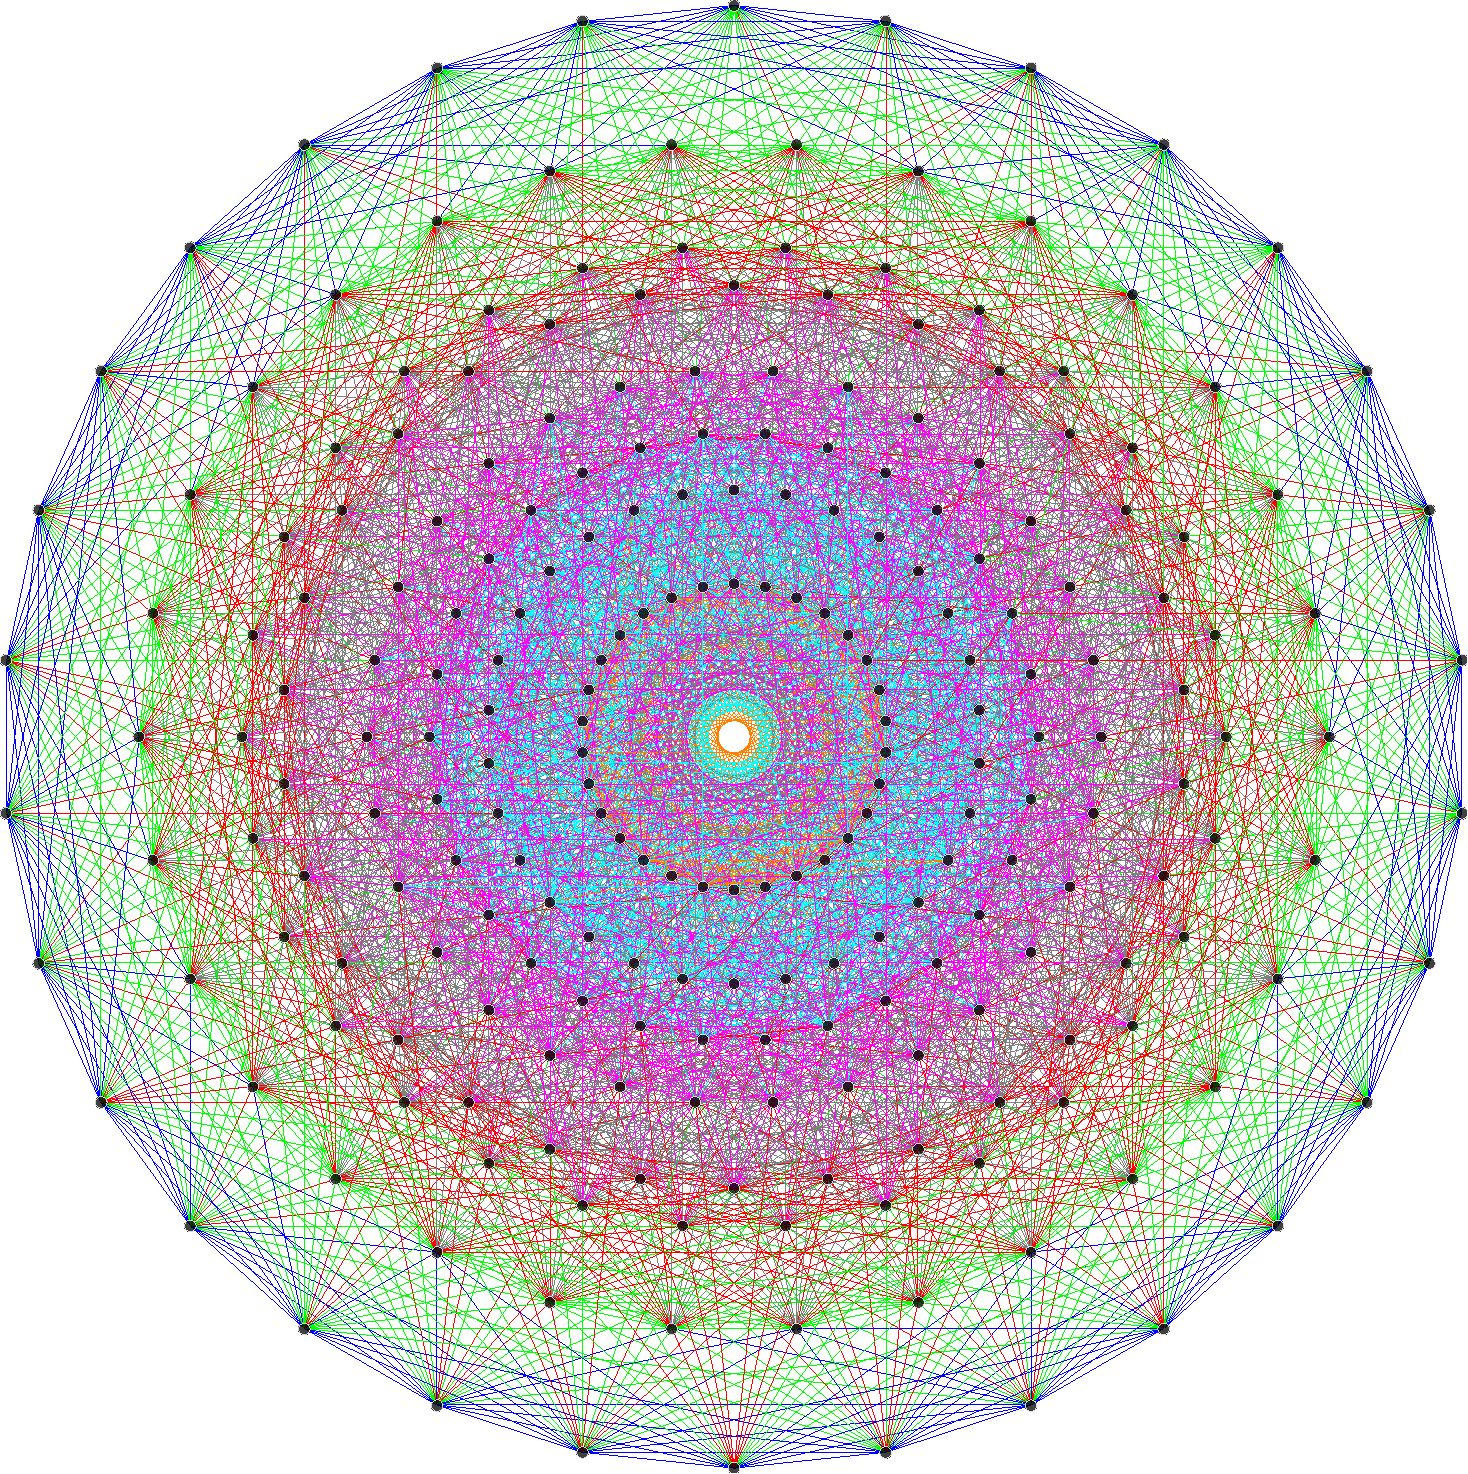
\includegraphics[width=.85\textwidth]{e8graph.pdf}}

\begin{document}
\pagenumbering{Alph}
\maketitle % 打印标题
\frontmatter
\chapter{Preface}
Mainly refer to\cite{Hall-Lie-2013}.

\tableofcontents

\mainmatter{}
\chapter{Lie Group}

\begin{definition}[Lie group]%
    \label{def: Lie group}
    Let $G$ be a smooth manifold and also a group. 
    If the group multiplication $\cdot \colon G^2 \to G; g, f \mapsto gf$ 
    and the inversion $G \to G; g \mapsto g^{-1}$
    are both smooth, then we call $G$ a \indexbf{Lie group}.
\end{definition}



\begin{definition}[Lie algebra]%
    \label{def: Lie algebra}
    Let $G$ be a Lie group, $e \in G$ be the identity of $G$.
    The \indexbf{Lie algebra} $\indexmath[g]{\mathfrak g} = T_e G$ of Lie group $G$ is the tangent space of $G$ at $e$, equipped with a bracket operation $[,] \colon \mathfrak g^2 \to \mathfrak g$ s.t.\ 
    \begin{equation*}
        [v, w] = [V, W] \vert_{e},
    \end{equation*}
    where $V, W$ are two left-invariant vector fields that $V_e = v$ and $W_e = w$.
\end{definition}



\appendix
\chapter{Appendix}

\backmatter{}
\nocite{*} % 这个表示列出所有没有在文中被引用的参考文献
\printbibliography[heading=bibliography, title={Bibliography}]

\indexprologue{Here listed the important symbols used in this notes.}
\printindex[symbol]

\printindex

\end{document}